\documentclass{article}
\usepackage[UTF8]{ctex}
\setmainfont{Calibri Light}
\usepackage{setspace}
\renewcommand{\baselinestretch}{1.2}
\usepackage{amsmath,bm}
\usepackage{framed} 
\usepackage{wrapfig}
\usepackage{amssymb}
\usepackage{ntheorem}
\usepackage{graphicx}
\usepackage{bbm}
\usepackage{hyperref}
\hypersetup{
	colorlinks=true,
	linkcolor=blue,
	filecolor=cyan,      
	urlcolor=red,
	citecolor=green,
}
\newtheorem{theorem}{Theorem}
\newtheorem{corollary}{Corollary}
\newtheorem{lemma}{Lemma}
\newtheorem*{proof}{Proof}
\setlength{\parindent}{2em}
\author{Siheng Zhang\\zhangsiheng@cvte.com}
\title{Chapter \textbf{\textit{4}} Linear Model}
\date{\today}
\usepackage[a4paper,left=18mm,right=18mm,top=25mm,bottom=25mm]{geometry} 

\begin{document}
\maketitle  

This part corresponds to \textbf{Chapter 1,3,4 of PRML, Chapter of UML}, and mainly answers the following questions:

\begin{itemize}
\item 
\end{itemize}

\tableofcontents
\newpage

	In linear regression model, the model is the same except that the learning target $y$ is continuous but not discrete. And the learning goal is the sum-of-square (SSE) loss

	\begin{equation}
	\min_\mathbf{w} L_S(h) =\sum_{i=1}^m  l(h(\mathbf{x}_i)) = \sum_{i=1}^m (h(\mathbf{x}_i) - y_i)^2 = \sum_{i=1}^m (\mathbf{w}^\top\mathbf{x}_i - y_i)^2 
	\end{equation}

	Suppose the fitting error $\epsilon_i = y_i-\mathbf{wx}_i$ is Gaussian noise, i.e., $\epsilon_i \sim\mathcal{N}(0,\beta)$. Then the log likelihood function of the training sequence is
	
	\begin{equation*}
	\log \mathcal{L} = -\frac{m}{2} \log 2\pi\beta - \sum_{i=1}^m \frac{(y_i-\mathbf{w}^\top\mathbf{x}_i)^2}{2\beta}
	\end{equation*}
Obviously, MLE is equivalent to linear regression.

	\begin{framed}
	\begin{scriptsize}
	\begin{spacing}{1.2}
	\noindent\textit{\textbf{remark8.} Since linear regression is not a binary prediction task, we cannot analyse its sample complexity using the VC-dimension. One possible analysis of the sample complexity of linear regression is by relying on the "discretization trick". However, to apply the sample complexity bounds from Chapter 2 we also need that the loss function will be bounded.}
	\end{spacing}
	\end{scriptsize}
	\end{framed}
	
\section{Generalized linear regression}
	
	The model is just a linear function of the input variables, and this imposes significant limitations on it. Therefore, extended model considers \textbf{linear} combination of fixed \textbf{non-linear} functions of the input variables, of the form
	
	\begin{equation}
	h(\mathbf{x}) = w_0 + \sum_{j=1}^d w_j \phi_j(x)
	\end{equation}
where $\phi_j(x)$ are known as \textit{basis functions}. Again, denote $\phi_0(\mathbf{x})=1$ so that $h(\mathbf{x}) = \tilde{\mathbf{w}}^\top \phi(\mathbf{x})$. For Simplification, we also neglect the `tilde' symbol from now on.

	Least squares also gives the result by $\mathbf{w} = \Phi^\dag \mathbf{y} = (\Phi^\top \Phi)^{-1} \Phi^\top \mathbf{y}$. $\Phi$ is an $n*d$ matrix, whose elements are given by $\Phi_{nj} = \phi_j(\mathbf{x}_n)$.

	\begin{framed}
	\begin{scriptsize}
	\begin{spacing}{1.2}
	\noindent\textit{\textbf{remark9: multiple-outputs.} The solution to multiple-outputs regression problem decouples between the different target variables so we do not need to discuss it here.}
	
	\noindent\textit{\textbf{remark10: on-line learning.} Batch techniques involve processing the entire training set in one go, can be computationally costly for large data sets. For linear regression, stochastic gradient descent algorithm updates parameter using $\mathbf{w}^{t+1}=\mathbf{w}^{t} - lr*\nabla L_{(\mathbf{x}_t,y_t)}(h) = \mathbf{w}^{t} + lr* (y_i - (\mathbf{w}^t)^\top \mathbf{\phi} (\mathbf{x}_t)) \mathbf{\phi} (\mathbf{x}_t)$, in which $lr$ is the learning rate.}

	\noindent\textit{\textbf{remark11: Basis function examples.}} 1. \textbf{Polynomial basis}, 2. \textbf{Radical basis}, 3. \textbf{Fourier basis}.
	
	\end{spacing}
	\end{scriptsize}
	\end{framed}
	
\section{Regularization \textit{a.k.a} Bayesian linear regression}
	
	In closed-form solution, if $n\leq d$, the SSE loss can achieve zero. It means that the model is able to 'memorize' all training examples, but the parameters vary significantly if the data points changes (even just a bit). So if there exists noisy data point, the model fits the noise well (zero training error) and will show bad performance to unseen data. This phenomenon is called \textbf{over-fitting}. Formally, consider the expected loss with squared error,
	\begin{equation*}
	\begin{split}
	\mathbb{E}(l) &= \int \int l(h(\mathbf{x})) p(\mathbf{x}, y) \text{d} \mathbf{x} \text{d}y \\
	&= \int \int (h(\mathbf{x})-y)^2 p(\mathbf{x}, y) \text{d} \mathbf{x} \text{d}y
	\ \ \ \ \footnotesize{\text{Note that, setting its derivatives to zero leads to $h(\mathbf{x}) = \int yp(\mathbf{x}, y) \text{d} y /p(\mathbf{x}) = \mathbb{E}(y|\mathbf{x})$}}\\
	&= \int \int \left\{ h(\mathbf{x}) - \mathbb{E} (y|\mathbf{x}) + \mathbb{E} (y|\mathbf{x}) - y \right\}^2 p(\mathbf{x}, y) \text{d} \mathbf{x} \text{d}y \\
	&= \int \left\{ h(\mathbf{x}) - \mathbb{E} (y|\mathbf{x}) \right\}^2 p(\mathbf{x}) \text{d} \mathbf{x} + \int \int \left\{\mathbb{E} (y|\mathbf{x}) - y \right\}^2 p(\mathbf{x}, y) \text{d} \mathbf{x} \text{d} y
	\end{split}
	\end{equation*}
	%&= \int \int \left\{ \left[ h(\mathbf{x}) - \mathbb{E} (y|\mathbf{x}) \right]^2 + \left[\mathbb{E} (y|\mathbf{x}) - y \right]^2 + 2 \left[ h(\mathbf{x}) - \mathbb{E} (y|\mathbf{x}) \right] \left[\mathbb{E} (y|\mathbf{x}) - y \right]  \right\} p(\mathbf{x}, y) \text{d} \mathbf{x} \text{d}y \\
	
	The second term, which is independent of $h(\mathbf{x})$, arises from the intrinsic noise on the data and represents the minimum achievable value of the expected loss. The first term depends on our choice for the function $h(\mathbf{x})$. Because it is non-negative, its optimal value is zero. If we had an unlimited supply of data (and unlimited computational resources), we could in principle find the regression function $h(\mathbf{x})$ to any desired degree of accuracy. But indeed, we can just estimate $h(\mathbf{x})$ from a particular data set $\mathcal{D}$, so we turn to study the following:
	
	\begin{equation}
	\begin{split}
	\mathbb{E}_\mathcal{D} \left[ \left\{ h(\mathbf{x};\mathcal{D})- \mathbb{E}(y|\mathbf{x}) \right\}^2 \right]
	&= \mathbb{E}_\mathcal{D} \left[  \left\{ h(\mathbf{x};\mathcal{D})- \mathbb{E}_\mathcal{D}(h(\mathbf{x};\mathcal{D})) + \mathbb{E}_\mathcal{D}(h(\mathbf{x};\mathcal{D})) - \mathbb{E}(y|\mathbf{x}) \right\}^2 \right] \\
	&= \mathbb{E}_\mathcal{D} \left[ \left\{ \mathbb{E}_\mathcal{D}(h(\mathbf{x};\mathcal{D})) - \mathbb{E}(y|\mathbf{x}) \right\}^2 \right] + \mathbb{E}_\mathcal{D} \left[ \left\{ h(\mathbf{x};\mathcal{D})- \mathbb{E}_\mathcal{D}(h(\mathbf{x};\mathcal{D}))\right\}^2 \right] \\
	&= \underbrace{\left\{ \mathbb{E}_\mathcal{D}(h(\mathbf{x};\mathcal{D})) - \mathbb{E}(y|\mathbf{x}) \right\}^2}_{\text{bias}^2} + \underbrace{\mathbb{E}_\mathcal{D} \left[ \left\{ h(\mathbf{x};\mathcal{D})- \mathbb{E}_\mathcal{D}(h(\mathbf{x};\mathcal{D}))\right\}^2 \right]}_{\text{variance}}
	\end{split}
	\end{equation}
The first term, called the squared bias, represents the extent to which the average prediction over all data sets differs from the desired regression function. The second term, called the variance, measures the extent to which the solutions for individual data sets vary around their average, and hence this measures the extent to which the regressor is sensitive to the particular choice of data set.

	As discussed before, there is a trade-off between bias and variance: flexible models having low bias and high variance, and relatively rigid models having high bias and low variance. Bayesian linear regression set a prior assumption of $\mathbf{w}$, and view the learning procedure to maximizing its posterior. Two of the most popular case is discussed below. 

\subsubsection{Ridge regression}
	\begin{wrapfigure}{r}{5cm}
	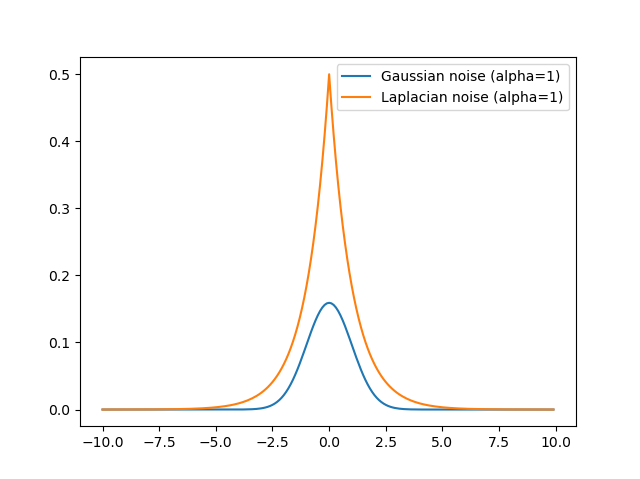
\includegraphics[scale=.3]{C4-1.png}	
	\title{\small{Laplace distribution and Gaussian distribution with $\alpha=1$.}}
	\end{wrapfigure}
	Ridge regression addresses on over-fitting by penalizing the $l_2$-norm of weight vector,
	
	\begin{equation*}
	\min_\mathbf{w} \sum_{i=1}^m (\mathbf{w\phi}_i(\mathbf{x}) - y_i)^2 + \lambda\|\mathbf{w}\|^2_2
	\end{equation*}

	If we assume a Gaussian prior for the weight vector, $\mathbf{w}\sim\mathcal{N}(0,\alpha^{-1}\mathbf{I})$,  the posterior of the training sequence is:
	
	\begin{equation}
	p(\mathbf{w}|S) \propto p(\mathbf{w}) p(S|\mathbf{w}) \propto \exp \left( -\frac{\alpha}{2} \mathbf{w}^\top \mathbf{w} \right) \cdot \prod_{i=1}^N \exp \left( -\frac{(y_i-\mathbf{wx}_i)^2}{2\beta} \right) 
	\end{equation}
	
Maximizing the log posterior function is equivalent to the ridge regression.
	
	
\subsubsection{Lasso}

	Lasso addresses on over-fitting by penalizing the $l_1$-norm of weight vector,
		
	\begin{equation*}
	\min_\mathbf{w} \sum_{i=1}^m (\mathbf{w\phi}_i(\mathbf{x}) - y_i)^2 + \lambda\|\mathbf{w}\|_1
	\end{equation*}
	
	If we assume a Laplace prior for the weight vector, $p(\mathbf{w})=\frac{1}{2\alpha} \exp \left( -\frac{\|\mathbf{w}\|_1}{\alpha} \right)$, then the posterior is:
	
	\begin{equation}
	p(\mathbf{w}|S) \propto p(\mathbf{w}) p(S|\mathbf{w}) \propto \exp \left( -\frac{\|\mathbf{w}\|_1}{\alpha} \right) \cdot \prod_{i=1}^N \exp \left( -\frac{(y_i-\mathbf{wx}_i)^2}{2\beta} \right)
	\end{equation}

Maximizing the log posterior function is equivalent to the Lasso model.

	
	
\section{Predictive distribution}
	
\section{Equivalent kernel}

\end{document}